\section{Qt}
%short introduction to the chapter
Qt, pronounced "cute", is an open source cross-platform framework, mostly used for GUI(graphical user interface) programming. Qt has an easy to (re)use API(application programming interface), which in return gives high developer productivity. QT is C++ class library, hence new developers using Qt should have some understanding of C++.
This chapter introduces terminologies used in Qt, and tries to give some general insight to how Qt operates and works regarding GUI development.  

%Maybe something about licencing and version used.


%somewhere here should the "simple" inheritance diagram be.

\subsection{Qt Class Hierarchy and Object Model}
\label{sec:QtClassHierarchyAndObjectModel}
Qt broadly uses inheritance to create subclasses of instances in a natural way. QObject is the most basic class in Qt, see FIGURE. A lot of classes inherit from QObject, like QWidget, which is the base of all user interface objects. 
C++ offers efficient runtime for a object oriented scheme, but lacks in regard to flexibility due to the static nature of the C++ Object Model. Qt has implemented the QObject as the hearth of the Qt Object Model, which preserve the efficient runtime while also offering more flexibility for the GUI domain. The Qt Object Model is implemented with standard C++ techniques. Some of the features that the Qt Object Model adds are e.g.

\begin{itemize}
\item Inter-Object Communication called Signal and Slots in the Qt Object Model. This topic is expanded upon in section~\ref{sec:signalandslots}.
\item Object Trees which structures ownership of objects in a natural fashion. This topic is expanded upon in section~\ref{sec:qwidgets}.
\end{itemize}

\subsubsection{The Meta-Object System}
Due to the Qt Object Model the Meta-Object System was in turn created, which on the bottom line provides the Signal and Slots for inter-object communication and other features from the the QT Object Model. The Meta-Object System is based on three things:
\begin{enumerate*}[label={\alph*)},font={\color{red!50!black}\bfseries}]
\item the QObject class
\item the Q\_OBJECT macro and
\item the Meta-Object compiler(moc).
\end{enumerate*}
Each QObject or subclass of QObject has an instance of QMetaObject created to hold the meta-data information, e.g. the name of the class or the class's meta-methods(signal, slots and other member functions). The Q\_OBJECT macro helps and defines the meta data for the moc at compile time. Please refer to figure~\ref{fig:QtC++BuildProcess} to see influence of the Meta-Object System in compile time.

\begin{figure}[h]
	\centering
	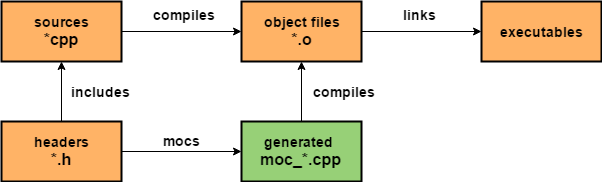
\includegraphics[scale=0.55]{Figures/QtC++BuildProcess.png}
	\caption{This figure shows how the the Meta-Object System is integrated at compile time. The yellow boxes indicate the normal C++ compiling procedure, whereas the green box is the added moc, which is compiled into the object files}
	\label{fig:QtC++BuildProcess}
\end{figure}

\subsection{QWidgets}
\label{sec:qwidgets}
QWidget is the base of all user interface objects(buttons, menus etc.). QWidget handles all events from the system the application is running on, i.e. In Qt, events are QEvent objects which is created upon outside activity (like a click on a mouse). Subclasses of QEvent involve more parameters to characterize a certain event, e.g. mousePressEvent(QMouseEvent* event). The event object is then sent to a specific QWidget object (maybe a button) and the QWidget handles the event with the according event handler.\\
As mentioned in~\ref{sec:QtClassHierarchyAndObjectModel} ownership of objects is structured in a tree, this means that a QWidget can have QWidget's within it self, see figure~\ref{fig:QWidgetExample}. A QWidget with no parent is called a top-level widget, which means the QWidget is an independent window. An instance like QWidget subclass QDialog(a pop up dialog window) is a top-level widget. QDialog can be instantiated with a parent, but the QDialog is still a top-level widget in this case, though the position of the dialog window is now centred relative to the parent.

\begin{figure}[h]
	\centering
	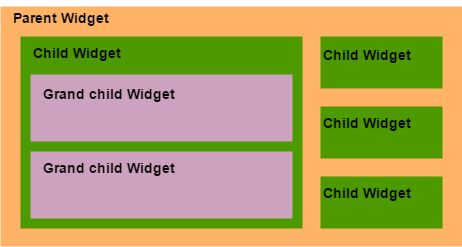
\includegraphics[scale=0.55]{Figures/QWidgetExample.png}
	\caption{Qt structures ownership of objects in a parent child relationship. The diagram shows a parent widget with various child widgets in a layout, more on layouts in section~\ref{sec:QLayout}.}
	\label{fig:QWidgetExample}
\end{figure}

When a QWidget is used as a container to hold and group children, the QWidget is called a composite widget. A parent widget is clipped to the size that it children requires, though this can be changed in the widget's size policy. 


Subclasses of QEvent involve more parameters to characterize a certain event.

events -> QEvent eventhandling -> mousePressEvent() e.g.
%events vs signal and slots

\subsection{QMainWindow}
QMainWindow -> framework for application's user interface. REF TO FIGURE
QMenuBar -> pulldown menu items
QToolBar -> moveable panels
QDock -> docked or top-level window
Central Widget -> RWStudioView3D -> openGL

\subsection{QLayout}
\label{sec:QLayout}
Arrange child widgets within a widget
Updates when contents change
QHBoxLayout example. CODE AND PICTURE OF LAYOUT

\subsection{Signal and Slots}
\label{sec:signalandslots}
Communication -> objects
Alternative to callback -> explain callback
Signal and slots -> connect() RET TO FIGURE
Signal -> 
Slot -> normal function (only special thing is it can be connected to a signal) -> found by moc
\subsubsection{Difference between events and Signal/Slots}


\subsection{Subclassing}

\subsection{Plug-in}

